\chapter{Proposed Methodology}
\label{ch:4}
This chapter gives the method the thesis set out to evaluate, the change of setting that turned out
to matter, the data all of it is measured on, and how the whole grid was implemented and run.
\section{Design Process or Methodology Overview}
\label{sec:4.overview}
The design proceeds in four steps. The method is built exactly as the literature proposes it, a
committee of task-adapted teachers weighted per instance by reliability
(Section~\ref{sec:4.design}). It is measured against the control that literature omits, the same
student trained with no teacher, over a grid of students, committees, objectives and seeds. Whatever
that grid shows, its cause is then established by measurement rather than by argument, on the
teachers themselves rather than on the students they train (Section~\ref{sec:5.2}). And where the
cause points, the setting is changed and measured again, with the predictions written down before
each run. Figure~\ref{fig:schematic} shows the distinction the last step turns on: in both settings
the same teacher and the same student are used, and only the text on which the student imitates the
teacher differs.
\begin{figure}[htbp]
\centering
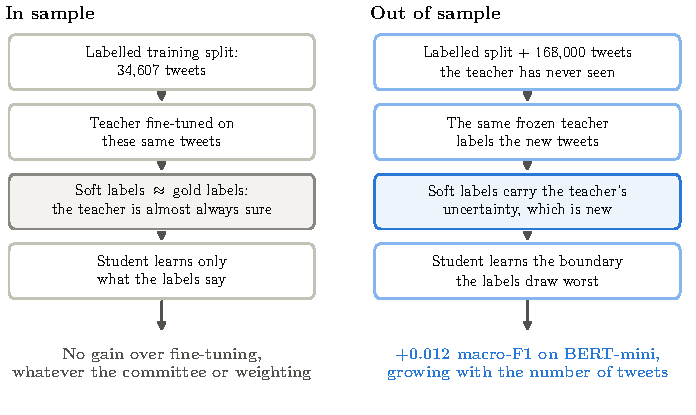
\includegraphics[width=\textwidth]{figures/fig_schematic.pdf}
\caption[In-sample against out-of-sample distillation]{In-sample against out-of-sample distillation. The same teacher and student are used in both settings; only the text on which the student imitates the teacher differs. In sample, on the tweets the teacher was fine-tuned on, its soft labels repeat the gold labels; out of sample, on tweets it has never seen, they carry its uncertainty.}
\label{fig:schematic}
\end{figure}
\section{Preliminary Design or Design (Model) Specification}
\label{sec:4.design}
Sections~\ref{sec:3.1} to~\ref{sec:3.4} define the committee, the per-instance weighting, the
objective and the specialist teacher exactly as they were audited; Section~\ref{sec:3.5} defines
in-sample and out-of-sample distillation and their controls; Section~\ref{sec:3.6} states what is
measured about the weighting; and Section~\ref{sec:3.7} gives the training procedure as an
algorithm.
\subsection{Notation and Committee}
\label{sec:3.1}
Let $x_i$ be a text with majority label $y_i \in \{1,\dots,C\}$. A committee of $K$ teachers
produces logits $z_k(x_i) \in \mathbb{R}^C$ and masked-mean-pooled last-layer states $h_k(x_i) \in
\mathbb{R}^{d_k}$; the student produces $z_s(x_i)$ and $h_s(x_i) \in \mathbb{R}^{d_s}$, pooled the
same way, which for the BiLSTM student is the masked mean of its top-layer bidirectional states
($d_s = 512$), so the hidden-state term is defined identically for every student; plus an auxiliary
irony head $z_s^{\text{irony}}(x_i) \in \mathbb{R}^2$ whose target $z_{\text{irony}}(x_i) \in
\mathbb{R}^2$ comes from the irony checkpoint \emph{before} task adaptation, in its own irony
against non-irony label space. $W_k \in \mathbb{R}^{d_k \times d_s}$ is a learned projection from
the student width to teacher $k$'s width; $T$ is the distillation temperature and $\tau$ the weight
temperature; $E$ is the number of epochs and $B$ the batch size. All sums over $j$ or $k$ run over
the $K$ teachers.

Teachers are \emph{task-adapted}: each is initialised from a specialist checkpoint and fine-tuned on
the target training split, so that every committee member shares the task's label space. Without
this step a sarcasm model's logits are not comparable with an abuse model's and cannot enter a KL
term. The homogeneous committee $\mathcal{K}_{\text{homo}}$ is BERT-large \cite{devlin2019bert},
HateBERT \cite{caselli2021hatebert} and a Twitter irony RoBERTa \cite{barbieri2020tweeteval,
liu2019roberta}: a general encoder, a specialist in abuse that says what it means, and a specialist
in saying one thing and meaning another. The heterogeneous committee adds DeBERTa-v3-base
\cite{he2023debertav3}. The third committee adds the implicit specialist of Section~\ref{sec:3.4}.
Teachers are frozen after adaptation and their outputs cached once on every split the student will
train on; the student never sees a teacher at run time.

Table~\ref{tab:symbols} lists every symbol used in this chapter, with the set it is drawn from and
the value it takes in the runs reported here; Sections~\ref{sec:3.2} to~\ref{sec:3.5} define each one
where it is introduced.

\begin{table}[htbp]
\centering
\footnotesize
\caption[Symbols used in Chapter 3]{Every symbol of this chapter, the set it is drawn from, and the
value or range it takes in the runs of Chapter~\ref{ch:5}.}
\label{tab:symbols}
\begin{adjustbox}{max width=\textwidth}
\begin{tabular}{llll}
\toprule
Symbol & Meaning & Domain & Value or range used \\
\midrule
$x_i$ & a text & strings & tweets, truncated to 128 word pieces \\
$y_i$ & its majority label & $\{1,\dots,C\}$ & one of six classes \\
$C$ & number of classes & $\mathbb{N}$ & 6 on tweets, 3 on the implicit benchmark \\
$K$ & number of teachers & $\mathbb{N}$ & 3 or 4 \\
$B$ & batch size & $\mathbb{N}$ & 32 \\
$E$ & epochs & $\mathbb{N}$ & 6; 13 and 35 in the matched-steps controls \\
$\mathcal{D}$ & labelled training split & set of texts & 34,607 tweets \\
$\mathcal{V}$ & validation split & set of texts & 4,326 tweets \\
$\mathcal{U}$ & unlabelled transfer set & set of texts & empty in sample; 5,000 to 205,593 out \\
$z_k(x_i)$ & teacher $k$'s logits & $\mathbb{R}^C$ & cached once, never updated \\
$h_k(x_i)$ & teacher $k$'s pooled state & $\mathbb{R}^{d_k}$ & masked mean of its last layer \\
$d_k$ & teacher $k$'s width & $\mathbb{N}$ & 768, or 1024 for BERT-large \\
$z_s(x_i)$ & student logits & $\mathbb{R}^C$ & updated every step \\
$h_s(x_i)$ & student pooled state & $\mathbb{R}^{d_s}$ & masked mean, pooled as the teachers are \\
$d_s$ & student width & $\mathbb{N}$ & 256 to 768; 512 for the BiLSTM \\
$z^{\mathrm{irony}}_s(x_i)$ & auxiliary head logits & $\mathbb{R}^2$ & discarded at inference \\
$z_{\mathrm{irony}}(x_i)$ & its target & $\mathbb{R}^2$ & from the irony checkpoint before adaptation \\
$W_k$ & projection student $\to$ teacher $k$ & $\mathbb{R}^{d_k \times d_s}$ & learned, discarded at inference \\
$T$ & distillation temperature & $(0, \infty)$ & 4; swept over $\{1, 2, 8\}$ \\
$\tau$ & weight temperature & $(0, \infty)$ & 1; swept over 0.05 to 5 \\
$\ell_k(i)$ & teacher $k$'s loss on $x_i$ & $[0, \infty)$ & 0.03 to 0.23 on $\mathcal{D}$ (Section~\ref{sec:5.6}) \\
$w_k(i)$ & in-sample weight of teacher $k$ & $(0,1)$, $\sum_k w_k(i) = 1$ & 0.318 to 0.356 on average \\
$\bar p(i)$ & the mixed soft target & simplex in $\mathbb{R}^C$ & near one-hot in sample \\
$m_i$ & label mask & $\{0, 1\}$ & 1 on $\mathcal{D}$, 0 on $\mathcal{U}$ \\
$\alpha, \beta$ & weight of the KL and hard terms & $[0, \infty)$ & 0.4 each; $\alpha$ swept over $\{0.2, 0.6\}$ \\
$\gamma$ & weight of the hidden-state term & $[0, \infty)$ & 0.2; 0 in the ablation \\
$\delta$ & weight of the irony term & $[0, \infty)$ & 0.3; swept over $\{0.1, 0.5\}$ \\
$\mathcal{L}_{\mathrm{KL}}, \mathcal{L}_{\mathrm{hid}}, \mathcal{L}_{\mathrm{irony}}, \mathcal{L}$ & the loss terms and their sum & $[0, \infty)$ & minimised by AdamW \\
$\nu$ & neighbours for the out-of-sample weight & $\mathbb{N}$ & 20 \\
$c_k(v)$ & is teacher $k$ correct on $v$ & $\{0, 1\}$ & measured on $\mathcal{V}$ \\
$r_k(x)$ & teacher $k$'s local accuracy & $(0, 1)$ & Laplace-smoothed, equation (3.7) \\
$w_k^{\mathrm{knn}}(x)$ & out-of-sample weight & $(0,1)$, $\sum_k w_k^{\mathrm{knn}}(x) = 1$ & within 0.03 of uniform \\
$\mathcal{K}_{\mathrm{homo}}, \mathcal{K}_{\mathrm{spec}}$ & the committees & sets of teachers & 3 and 4 members \\
\bottomrule
\end{tabular}
\end{adjustbox}
\end{table}

\subsection{Per-Instance Reliability}
\label{sec:3.2}
For each training instance the committee is weighted by how reliable each teacher is on it:

\begin{equation}
\ell_k(i) = \mathrm{CE}\big(z_k(x_i),\, y_i\big), \qquad
w_k(i) = \frac{\exp(-\ell_k(i)/\tau)}{\sum_{j} \exp(-\ell_j(i)/\tau)} .
\end{equation}

$w_k(i)$ is the posterior probability that teacher $k$ is the right expert for $x_i$ under a uniform
prior and a likelihood $p(y_i \mid k, x_i)^{1/\tau}$: at $\tau = 1$ it is Bayesian model averaging
over the committee on that instance; $\tau \to \infty$ recovers uniform averaging and $\tau \to 0$
hard selection of the single best teacher. Per-batch weighting, as in earlier work, replaces
$\ell_k(i)$ by its batch mean. Because the teachers are frozen and cached, $w_k(i)$ is a fixed
function of the data: it varies across instances and never across epochs or seeds, so ``dynamic''
means instance-adaptive and nothing else.
\subsection{Objective}
\label{sec:3.3}
\begin{equation}
\bar p(i) = \sum_k w_k(i)\, \mathrm{softmax}\!\big(z_k(x_i)/T\big),
\end{equation}

\begin{equation}
\mathcal{L}_{\mathrm{KL}}(i) = T^2\, \mathrm{KL}\!\big(\bar p(i)\,\|\,\mathrm{softmax}(z_s(x_i)/T)\big),
\end{equation}

\begin{equation}
\mathcal{L}_{\mathrm{hid}}(i) = \sum_k \frac{w_k(i)}{d_k}\, \big\| W_k h_s(x_i) - h_k(x_i) \big\|_2^2,
\end{equation}

\begin{equation}
\mathcal{L}_{\mathrm{irony}}(i) = T^2\, \mathrm{KL}\!\big(\mathrm{softmax}(z_{\text{irony}}(x_i)/T)\,\|\,\mathrm{softmax}(z_s^{\text{irony}}(x_i)/T)\big),
\end{equation}

\begin{equation}
\mathcal{L} = \frac{\alpha}{B}\sum_i \mathcal{L}_{\mathrm{KL}}(i)
 + \beta\, \frac{\sum_i m_i\, \mathrm{CE}(z_s(x_i), y_i)}{\sum_i m_i}
 + \frac{\gamma}{B}\sum_i \mathcal{L}_{\mathrm{hid}}(i) + \frac{\delta}{B}\sum_i \mathcal{L}_{\mathrm{irony}}(i),
\end{equation}

with $\alpha = \beta = 0.4$, $\gamma = 0.2$, $\delta = 0.3$, $T = 4$ and $\tau = 1$ unless stated,
and $m_i \in \{0, 1\}$ a label mask that is 1 on labelled rows and 0 on the unlabelled rows of
Section~\ref{sec:3.5}. Every symbol in these five equations appears in Table~\ref{tab:symbols} with
the set it is drawn from and the value it takes here. The hard-label term is averaged over the
labelled rows of the batch, not over the batch, so appending unlabelled rows does not silently
dilute supervision: the ratio of the two terms is the same in every arm of Section~\ref{sec:5.8}.
The irony target comes from the irony checkpoint before adaptation, whose label space is irony
against non-irony and cannot enter the committee's KL term, so it is distilled into a second head on
the student's pooled state; the head is discarded at inference and exists to shape the shared
representation. The same checkpoint, after task adaptation into the six-class label space, is the
committee's third member. Uniform multi-teacher distillation sets $w_k(i) = 1/K$; single-teacher
distillation uses BERT-large alone; fine-tune-only drops every teacher term and trains on the
cross-entropy alone. Training: 6 epochs, AdamW \cite{loshchilov2019decoupled} at $3 \times 10^{-5}$
($10^{-3}$ for the BiLSTM), 10 per cent warm-up and linear decay, batch 32, gradient clipping at
1.0, mixed precision on GPU, best validation macro-F1 epoch kept, early stopping with patience 2,
implemented in PyTorch and Transformers \cite{paszke2019pytorch, wolf2020transformers}; the
remaining settings are collected in Appendix~\ref{app:hyper}.
\subsection{The Implicit Specialist and Its Controls}
\label{sec:3.4}
No public checkpoint and neither established corpus holds knowledge of abuse by implication, so a
committee assembled from them cannot route to it. We therefore train the fourth member: HateBERT
fine-tuned on the implicit benchmark of Section~\ref{sec:4.2}, then task-adapted onto the tweet
corpus like every other teacher, its classification head re-initialised for the six-class label
space. It forms its own committee, $\mathcal{K}_{\text{spec}} = \mathcal{K}_{\text{homo}} \cup
\{\text{specialist}\}$, so that its effect is a three-seed comparison of two full committees rather
than a single ablation. Two controls accompany it, fixed before it was trained. The first distils
from the specialist alone, asking whether the committee contributes anything the specialist does
not. The second fine-tunes the same student on the implicit corpus and then on the tweet task with
no teacher, asking whether the knowledge, if any arrives, came from distillation or from the data.
\subsection{In Sample and Out of Sample}
\label{sec:3.5}
Every objective above is evaluated in two settings that differ only in where the teacher's function
is sampled. \emph{In sample}, the student is trained on the labelled split $\mathcal{D}$, the
teachers' outputs are cached on $\mathcal{D}$, and $\mathcal{D}$ is the split the teachers were
fine-tuned on. \emph{Out of sample}, an unlabelled transfer set $\mathcal{U}$ of texts outside every
teacher's training split is appended to $\mathcal{D}$; on $x_u \in \mathcal{U}$ the label mask $m_u
= 0$ removes the hard-label term, and the student trains from $\alpha\, \mathcal{L}_{\mathrm{KL}}(u)
+ \gamma\, \mathcal{L}_{\mathrm{hid}}(u) + \delta\, \mathcal{L}_{\mathrm{irony}}(u)$ alone. Nothing
else changes: the same objective, teachers, student, epochs and learning rate, and the hard-label
term stays averaged over the labelled rows, so its weight against the teacher terms is the same in
every arm. The construction of $\mathcal{U}$ is in Section~\ref{sec:4.4}; it is shuffled once with a
fixed seed so that its prefixes are nested subsets, which is what lets Section~\ref{sec:5.8} vary
its size with everything else fixed.

Two controls separate what the soft labels carry from what more text and more updates carry. The
\emph{hard-label} control replaces $\bar p(u)$ by the committee's $\arg\max$ and trains the transfer
rows with cross-entropy alone. The \emph{matched-steps} controls fine-tune the student with no
teacher for as many updates as a transfer arm takes (13 epochs for the 42,013-row set, 35 for the
168,000-row set), early stopping off and the best validation epoch kept, so that optimisation length
is held equal rather than argued away.

Out of sample, the reliability of Section~\ref{sec:3.2} has no label to be scored against, so we
also test a reliability the teachers cannot have memorised. Let $\mathcal{V}$ be the validation
split, $c_k(v) \in \{0, 1\}$ whether teacher $k$ is correct on $v \in \mathcal{V}$, and $N_k(x)$ the
$\nu$ validation texts nearest $x$ by cosine similarity in teacher $k$'s own pooled space. Then

\begin{equation}
r_k(x) = \frac{1 + \sum_{v \in N_k(x)} c_k(v)}{\nu + 2}, \qquad
w_k^{\mathrm{knn}}(x) = \frac{r_k(x)^{1/\tau}}{\sum_j r_j(x)^{1/\tau}},
\end{equation}

with $\nu = 20$ and $\tau = 1$: the weight is proportional to the teacher's local out-of-sample
accuracy. In an out-of-sample run it replaces $w_k(i)$ on every row, labelled and unlabelled alike,
because the in-sample estimate is saturated on the labelled ones. Two caveats belong here rather
than in the results. The validation split is also the split each teacher's checkpoint was selected
on, so $c_k(v)$ is measured on data the teacher has seen once, and the estimate is optimistic; and
the signal is a control, not a proposal, whose ceiling Section~\ref{sec:5.4} sets before any student
trains on it.
\subsection{What Is Measured About the Weighting}
\label{sec:3.6}
A committee of specialists is only a committee if the weights go somewhere. For each teacher we
report the \emph{routing contrast}: its mean weight on instances of the class that holds indirect
abuse minus its mean weight on the classes that name their target, with a percentile bootstrap
interval over 2,000 resamples, measured in the committee the students actually trained with. With
tens of thousands of training instances almost any contrast excludes zero, so its size is read
against the uniform weight $1/K$. And because the weights are a fixed function of the data, the
sweep over $\tau$ reaches 0.05, where they are as sharp as the reliability signal allows.

\subsection{Training Procedure}
\label{sec:3.7}
Algorithm~\ref{alg:training} gives the procedure shared by every run. In-sample runs use an empty
transfer set; fine-tune-only runs skip the teachers and train on the labelled split with cross-entropy
alone.

\begin{algorithm}[htbp]
\caption{Distillation in and out of sample.}
\label{alg:training}
\begin{algorithmic}[1]
\Require labelled split $\mathcal{D}$; validation split $\mathcal{V}$; unlabelled transfer set
  $\mathcal{U}$, empty in sample; teacher checkpoints $M_1, \dots, M_K$; unadapted irony checkpoint
  $M_{\mathrm{irony}}$; pre-trained student $S$
\For{$k = 1, \dots, K$}
  \State fine-tune $M_k$ on $\mathcal{D}$, keep its best validation epoch, and freeze it \Comment{task adaptation}
\EndFor
\For{each text $x \in \mathcal{D} \cup \mathcal{U}$}
  \State cache $z_k(x)$ and $h_k(x)$ for every teacher $k$, and $z_{\mathrm{irony}}(x)$ from $M_{\mathrm{irony}}$
\EndFor
\If{the run weights out of sample}
  \State cache $h_k(v)$ and the correctness $c_k(v)$ for every $v \in \mathcal{V}$, and build each
    teacher's neighbour index \Comment{for equation (3.7)}
\EndIf
\State set the label mask $m_x = 1$ for $x \in \mathcal{D}$ and $m_x = 0$ for $x \in \mathcal{U}$
\For{epoch $= 1, \dots, E$}
  \For{each minibatch drawn from $\mathcal{D} \cup \mathcal{U}$}
    \State compute $z_s(x)$, $h_s(x)$ and $z^{\mathrm{irony}}_s(x)$ for every $x$ in the minibatch
    \State weight the teachers by $w_k(x)$ of Section~\ref{sec:3.2} in sample, and by
      $w_k^{\mathrm{knn}}(x)$ of Section~\ref{sec:3.5} on every row of an out-of-sample run
    \State compute the loss of Section~\ref{sec:3.3} with the mask $m_x$ and update $S$ and $W_1, \dots, W_K$
  \EndFor
  \State evaluate macro-F1 on the validation split and keep the best epoch
\EndFor
\State \Return $S$, discarding the projections $W_k$ and the irony head
\end{algorithmic}
\end{algorithm}


\textbf{What it costs.} Counting one forward-and-backward pass of the student over one text as the
unit, and writing $c_k$ for the cost of one forward pass of teacher $k$ in the same unit, the
procedure divides into work done once and work done every epoch. Adapting the teachers is
$O\!\left(E_t \sum_k |\mathcal{D}|\, c_k\right)$ for $E_t = 5$ epochs, and caching their outputs over
$\mathcal{D} \cup \mathcal{U}$ is one further pass each, $O\!\left((|\mathcal{D}| + |\mathcal{U}|)
\sum_k c_k\right)$; both are paid once and reused by every student. An out-of-sample run adds the
neighbour search of equation (3.7), which is $O(K |\mathcal{V}| \bar d)$ to embed the validation split
and $O\!\left(K (|\mathcal{D}| + |\mathcal{U}|) |\mathcal{V}| \bar d\right)$ to query it exactly, for a
mean teacher width $\bar d$; with $|\mathcal{V}| = 4{,}326$ this is small beside the caching and is
also done once. Training the student is
$O\!\left(E (|\mathcal{D}| + |\mathcal{U}|)\big(1 + K C + K d_k d_s\big)\right)$: one student pass per
row, plus a $C$-way KL against each teacher and one $d_k \times d_s$ projection each, none of which
involves a teacher forward pass because the logits and states are cached. The teacher terms are
therefore a constant factor per row rather than a factor that grows with the student, and the only
term that grows with the recipe is $|\mathcal{U}|$: the cost is linear in the size of the transfer
set, which is what makes the curve of Section~\ref{sec:5.8} affordable and what sets its price, 18.4
GPU-hours for the whole grid. Inference is $O(1)$ in this unit and unchanged by any of it, since
$W_k$, the irony head and the teachers are all discarded.

\section{Data Collection}
\label{sec:4.data}
The primary benchmark is a cleaned fine-grained cyberbullying tweet corpus. A benchmark that labels
implication, built from a single corpus, and inference-only probe sets measure what the tweet corpus
cannot. An unlabelled transfer set, screened against all of them, supplies the out-of-sample text.
Each is described below with the cleaning, transformation and reduction applied to it, and
Section~\ref{sec:4.summary} summarises what survives.
\subsection{The Tweet Corpus}
\label{sec:4.1}
The fine-grained cyberbullying corpus \cite{wang2020sosnet} contains 47,692 tweets in six classes:
age, ethnicity, gender, religion, other\_cyberbullying and not\_cyberbullying. Repeated tweets are
common and some repeats carry different labels. We drop tweets shorter than two tokens (758), every
tweet whose normalised text appears with more than one label, all copies included (1,563 texts,
3,168 rows), and exact duplicates (507), then split the 43,259 survivors 80/10/10 stratified by
class with seed 42, asserting the splits disjoint on normalised text: 34,607 / 4,326 / 4,326. The
two classes that lose the most rows, other\_cyberbullying and not\_cyberbullying, are the two the
literature reports as confusable. A validation-to-test accuracy gap of 0.94 against 0.86 observed on
the raw corpus disappears on the cleaned split.

Table~\ref{tab:classes} gives the class distribution of the cleaned splits.

\begin{table}[htbp]
\centering
\small
\caption{Class distribution of the cleaned tweet corpus.}
\label{tab:classes}
\begin{tabular}{lrrrr}
\toprule
Class & Train & Validation & Test & Total \\
\midrule
age & 6,348 & 793 & 793 & 7,934 \\
ethnicity & 6,270 & 784 & 784 & 7,838 \\
gender & 6,020 & 753 & 753 & 7,526 \\
religion & 6,364 & 796 & 796 & 7,956 \\
other\_cyberbullying & 4,664 & 583 & 583 & 5,830 \\
not\_cyberbullying & 4,941 & 617 & 617 & 6,175 \\
\midrule
Total & 34,607 & 4,326 & 4,326 & 43,259 \\
\bottomrule
\end{tabular}
\end{table}

\subsection{The Implicit Benchmark}
\label{sec:4.2}
Neither the tweet corpus nor the Wikipedia corpus labels indirectness, so a model trained on either
never sees an example annotated as implicit. Two corpora annotate the distinction: the Implicit Hate
Corpus stage-1 release, 21,480 posts in three classes (not\_hate, explicit\_hate, implicit\_hate)
\cite{elsherief2021latent}, and ISHate, 28,763 original rows after excluding its augmentations and
its ToxiGen-sourced rows \cite{ocampo2023indepth}.

\textbf{The splits come from one corpus, and the reason is measured.} In the union, 95 per cent of
implicit examples come from the Implicit Hate Corpus and 89 per cent of explicit examples from
ISHate, and a TF-IDF classifier tells the two corpora apart at 0.91 macro-F1. A model trained on the
union can therefore score well on implicit-against-explicit by recognising the source. It also does
worse where it matters: on identical Implicit Hate test rows, a classical model trained on the union
reaches 0.473 F1 on implicit hate against 0.548 for the same model trained on that corpus alone,
while its aggregate macro-F1 is higher, 0.681 against 0.562, which is exactly the artefact. We
therefore build train, validation and test from the Implicit Hate Corpus and hold ISHate out whole
as a 27,096-row out-of-domain test set. Every text occurring in any probe set
(Section~\ref{sec:4.3}) is removed first, 1,581 rows across the two corpora, so that probe metrics
stay measured on text no model has trained on. Of those, 796 come from the Implicit Hate Corpus,
leaving 20,684; the tweet pipeline then removes 10 rows shorter than two tokens, 25 rows in 12 texts
carrying conflicting labels and 12 duplicates, and the remaining 20,637 are split 80/10/10 with seed
42 into 16,509 / 2,064 / 2,064, with training classes not\_hate 10,616, implicit\_hate 5,029,
explicit\_hate 864 and 108 explicit rows in the test split. ISHate loses the other 785 probe rows,
613 rows that also occur in those splits and 269 rows in 14 conflicting-label texts, which is how
its 28,763 become the 27,096 held out.

\textbf{The label is contested.} The two corpora share 629 texts. On whether a text is hateful at
all they agree on 99.7 per cent; on whether the hate is stated or implied they agree on 48.2 per
cent, the Implicit Hate Corpus labelling essentially all of the 624 shared hateful texts implicit
and ISHate labelling 324 explicit and 300 implicit. Two expert annotation efforts placing the
boundary in materially different places bounds how sharp any result on the implicit class can be,
and is the reason the benchmark's headline metric is a threshold-free ranking
(Section~\ref{sec:4.6}) rather than a decision. The benchmark is released as a build script plus a
per-row manifest (split, label, source, SHA-1 of the normalised text), so a reader can verify a
rebuild row by row without either party redistributing text.
\subsection{Probes}
\label{sec:4.3}
Three inference-only sets, never used for training by any model on any corpus. They are stored as
five files, because the benign-sarcasm probe keeps its unscreened and reviewed versions beside the
screened one the metrics use, and all five are screened against the transfer set. \emph{Benign
sarcasm}: 1,064 sarcastic tweets from iSarcasmEval \cite{abufarha2022semeval, oprea2020isarcasm},
author-labelled, of which 883 survive a screening pass over the rows a classical classifier flags as
abusive; the metric is the false-positive rate, the share whose argmax is any abusive class. Where a
score rather than a decision is needed, $p(\text{abusive})$ is one minus the probability of the
not-abusive class: one minus the probability of \texttt{not\_cyberbullying} on the tweet corpus, and
one minus the probability of \texttt{not\_hate} on the implicit benchmark. \emph{Ironic abuse}:
1,560 items, 797 posts labelled irony in the Implicit Hate Corpus stage-2 data and 763 original
ISHate rows labelled implicit; the metric is recall. \emph{Implicit abuse}: the 763 ISHate rows
alone. ISHate rows sourced from ToxiGen or the Implicit Hate Corpus are excluded from the probes so
that they stay independent of the corpus they test transfer into. The probes are rule-built from
published corpora, not hand-verified; a 300-item human annotation with inter-annotator agreement
\cite{fleiss1971measuring} is in progress. Probe metrics are only meaningful for models trained on
Twitter-domain data.
\subsection{The Transfer Set}
\label{sec:4.4}
The transfer set is unlabelled tweets the teachers have never fitted. Its base is abuse-domain text
from public corpora used as text only, their labels discarded before anything reads them: OLID
\cite{zampieri2019olid} and HatEval \cite{basile2019hateval} through TweetEval
\cite{barbieri2020tweeteval} (14,100 and 12,970 tweets), Davidson et al.
\cite{davidson2017automated} (24,783), and the 1,563 tweets of the cyberbullying corpus that our own
cleaning dropped for carrying more than one label. TweetEval's irony configuration is not used,
because it is the irony teacher's own fine-tuning data, and Founta et al. \cite{founta2018large} is
excluded under the provenance rule of Section~\ref{sec:4.5}. Every text is matched on the splits'
own normalised key against the train, validation and test splits, all five probe files and every
file of the implicit benchmark including the held-out ISHate set, and dropped on any hit; duplicates
within the set are dropped too. Of 53,416 texts, 318 are shorter than two tokens, 877 are
duplicates, 117 occur in a tweet split, 103 in the ironic- and implicit-abuse probes, 2 in the
implicit benchmark's test split and 9,988 in the held-out ISHate set, which incorporates HatEval's
tweets: \textbf{42,013 remain} (Davidson 24,139; OLID 13,760; HatEval 2,556; conflicting-label
tweets 1,558), 1.2 times the training split. The screen against ISHate matters: without it, a fifth
of the ``unlabelled'' set would have been text a later evaluation scores.

For the size curve the base set is extended with generic tweets from TweetEval's sentiment, emoji
and emotion configurations (59,899, 100,000 and 5,052 rows), screened identically and against the
base set itself: 163,580 survive (emoji 98,867, sentiment 59,715, emotion 4,998), giving 205,593
rows in all. The generic block is shuffled with the same seed before it is appended, so its sources
are mixed throughout rather than ordered by corpus. The base rows come first and verbatim, so a
prefix of the extended file up to 42,013 is the base set, prefixes below that are nested subsets of
it, and rows beyond it are generic. The size curve of Section~\ref{sec:5.8} uses the prefixes of
5,000, 10,000, 21,000, 42,013, 84,000 and 168,000 rows; the remaining 37,593 screened rows were
built and not used. Its composition control is the slice of the same file that follows the base set,
rows 42,013 to 84,026, which is 42,013 generic tweets and no abuse-domain text. The report of every
count (\texttt{transfer\_report.json}, \texttt{transfer\_big\_report.json}) is regenerated by the
run itself, with the same seed, from the same public sources; Appendix~\ref{app:transfer} says what
each file records.

Table~\ref{tab:transfer} records every count.

\begin{table}[htbp]
\centering
\small
\caption[Construction of the transfer set]{Construction of the transfer set. Upper part: rows read and kept per source. Lower part: rows
matching each screen; a row can match more than one screen, so the screens do not sum to the difference.}
\label{tab:transfer}
\begin{tabular}{lrr}
\toprule
Source & Rows read & Rows kept \\
\midrule
\multicolumn{3}{l}{\emph{Abuse-domain base set}} \\
OLID \cite{zampieri2019olid} & 14,100 & 13,760 \\
HatEval \cite{basile2019hateval} & 12,970 & 2,556 \\
Davidson et al. \cite{davidson2017automated} & 24,783 & 24,139 \\
Conflicting-label tweets of the corpus & 1,563 & 1,558 \\
Total & 53,416 & 42,013 \\
\midrule
\multicolumn{3}{l}{\emph{Generic extension}} \\
TweetEval sentiment & 59,899 & 59,715 \\
TweetEval emoji & 100,000 & 98,867 \\
TweetEval emotion & 5,052 & 4,998 \\
Total & 164,951 & 163,580 \\
\midrule
Extended set, base first & & 205,593 \\
\midrule
Screen & Base & Extension \\
\midrule
Shorter than two tokens & 318 & 114 \\
Duplicate within the set & 877 & 1,226 \\
Occurs in a tweet split & 117 & 14 \\
Occurs in a probe set & 103 & 0 \\
Occurs in the implicit benchmark's splits & 2 & 0 \\
Occurs in held-out ISHate & 9,988 & 9 \\
Occurs in the base set & -- & 8 \\
\bottomrule
\end{tabular}
\end{table}

\subsection{Summary of the Preprocessed Data}
\label{sec:4.summary}
Table~\ref{tab:data} is what survives every screen and is what the rest of the thesis is measured
on: 43,259 labelled tweets in six classes, split 80/10/10 and asserted disjoint on normalised text;
a 20,637-row implicit benchmark from one corpus with 27,096 rows of a second held out whole; three
inference-only probe sets no model trains on; and 205,593 unlabelled tweets, of which 42,013 are
abuse-domain and the rest generic, screened against every one of the sets above.

\begin{table}[htbp]
\centering
\small
\caption{The data used in this thesis.}
\label{tab:data}
\begin{tabular}{p{5.4cm}p{2.6cm}rrrp{1.5cm}}
\toprule
Set & Role & Train & Validation & Test & Labels \\
\midrule
Cyberbullying tweets, cleaned \cite{wang2020sosnet} & primary benchmark & 34,607 & 4,326 & 4,326 & 6 classes \\
Implicit Hate Corpus, single source \cite{elsherief2021latent} & implicit benchmark & 16,509 & 2,064 & 2,064 & 3 classes \\
ISHate, held out whole \cite{ocampo2023indepth} & out-of-domain test & -- & -- & 27,096 & 3 classes \\
Benign sarcasm probe \cite{abufarha2022semeval, oprea2020isarcasm} & inference only & -- & -- & 883 & -- \\
Ironic abuse probe \cite{elsherief2021latent, ocampo2023indepth} & inference only & -- & -- & 1,560 & -- \\
Implicit abuse probe, a subset of it \cite{ocampo2023indepth} & inference only & -- & -- & 763 & -- \\
Transfer set, abuse-domain base \cite{davidson2017automated, zampieri2019olid, basile2019hateval} & training, unlabelled & 42,013 & -- & -- & none \\
Transfer set, extended \cite{barbieri2020tweeteval} & training, unlabelled & 205,593 & -- & -- & none \\
\bottomrule
\end{tabular}
\end{table}

\section{Implementation of Selected Design}
\label{sec:4.impl}
\subsection{Teachers, Students, Floor}
\label{sec:4.5}
Teachers: BERT-large-uncased (335M), HateBERT (110M), Twitter-RoBERTa-base-irony (125M),
DeBERTa-v3-base (184M), and the implicit specialist (HateBERT, 110M), each fine-tuned on the tweet
training split for 5 epochs at $2 \times 10^{-5}$, batch 32, best validation epoch kept, trained
once. A provenance rule excludes from every test set, probe and transfer set any data a teacher's
checkpoint was trained on before adaptation. Students: BERT-mini (11.2M, the headline student),
BERT-small (28.8M) \cite{turc2019wellread}, DistilBERT (67.0M) \cite{sanh2019distilbert},
DeBERTa-v3-xsmall (70.8M) \cite{he2023debertav3}, and a two-layer BiLSTM over a WordPiece vocabulary
(10.4M) \cite{tang2019distilling}; the last two are the heterogeneous students. The classical floor
is TF-IDF over word 1-2 grams and character 3-5 grams with class-balanced logistic regression:
0.8798 macro-F1 on tweets, 0.5620 on the implicit benchmark (implicit\_hate F1 0.5562,
implicit-discrimination AUC 0.7610). Every neural result is read against it.
\subsection{Metrics}
\label{sec:4.6}
Recall on ironic abuse at a fixed threshold cannot distinguish a model that fails to see indirect
abuse from one that sees it and cannot separate it from harmless sarcasm. We report
\textbf{sarcasm-discrimination AUC}: the ROC-AUC of $p(\text{abusive})$ with the ironic-abuse probe
as positives and the benign-sarcasm probe as negatives, threshold-free and defined identically on
every corpus, with the recall-against-false-positive curve beside it because a deployment must
choose a threshold even though an evaluation should not. On the implicit benchmark the analogue is
\textbf{implicit-discrimination AUC}, implicit-hate rows against benign rows ranked by
$p(\text{implicit hate})$; macro-F1 there is dominated by an explicit class of 108 test rows and is
reported but not argued on. Elsewhere: macro-F1, accuracy, expected calibration error
\cite{guo2017calibration}, and per-class F1.
\subsection{Protocol and Statistics}
\label{sec:4.7}
Three seeds per main configuration, one for ablations, controls and sweeps. Every difference the
paper states is a paired bootstrap over the test set \cite{koehn2004statistical,
dror2018hitchhiker}: seeds paired by index, 1,000 resamples per seed, the 95 per cent interval of
the pooled differences. The grid makes 99 such comparisons and they are generated as a table, not
transcribed; nine intervals exclude zero, one for removing pre-training and eight for out-of-sample
distillation. A paired interval on 4,326 posts is about 0.014 wide, so the minimum detectable
difference is about 0.007 macro-F1 \cite{card2020power}, and we say so wherever a difference is
smaller. A pre-registered stop rule required at least one task-adapted teacher to beat the
fine-tune-only student on the clean test split before any distillation ran, and the predictions for
the three out-of-sample runs were written into the decision log before each ran and scored by a
script against the tables.

\textbf{One rule constrains every table.} The same code, data and seeds produce systematically
different results on a laptop CPU and on a Kaggle T4 (Section~\ref{sec:7.1}), so every number comes
from the Kaggle grid alone. Comparisons within it are valid because everything in it was trained
identically; numbers produced elsewhere are excluded rather than reconciled. The tweet grid is
complete: 179 student runs in 18.4 GPU-hours over the five Kaggle sessions that ran to completion.
The Wikipedia grid and the student grid on the implicit benchmark are not run and are named where
they would bear on a claim.

\subsection{Implementation and Compute}
\label{sec:4.8}
Every student and teacher in this thesis was trained on Kaggle T4 accelerators by one driver script that
resumes finished work from the previous session's output, so that the grid could grow across sessions
of at most twelve hours. Table~\ref{tab:sessions} lists the sessions of the tweet notebook. Two sessions
failed and are reported rather than hidden: the second stopped at teacher caching because the resume
logic had discarded the teacher weights, and the third froze inside a diagnostic cell until Kaggle ended
it; both faults were fixed, and the driver now kills any command that writes nothing for two hours. The
teachers, the implicit specialist and the student pre-trained on the implicit corpus were each trained
once and resumed by every later session. The code, the driver, the notebook and a CPU smoke test that runs
every stage on tiny models before any GPU session are in the repository.

\begin{table}[htbp]
\centering
\small
\caption{The Kaggle sessions of the tweet grid.}
\label{tab:sessions}
\begin{tabular}{clrr}
\toprule
Session & What it added & GPU-hours & Student runs, cumulative \\
\midrule
1 & the in-sample grid on five students and three committees & 8.24 & 120 \\
2 & failed at teacher caching; fixed & -- & 120 \\
3 & froze in a diagnostic cell; fixed & -- & 120 \\
4 & specialist committee, controls, sharpest temperatures & 1.41 & 131 \\
5 & the five out-of-sample arms & 2.11 & 146 \\
6 & the size curve and its first controls & 3.52 & 170 \\
7 & the 35-epoch control and two more students & 3.16 & 179 \\
\midrule
 & total of the completed sessions & 18.44 & 179 \\
\bottomrule
\end{tabular}
\end{table}
